<<<<<<< HEAD
\PassOptionsToPackage{unicode=true}{hyperref} % options for packages loaded elsewhere
\PassOptionsToPackage{hyphens}{url}
%
=======
<<<<<<< HEAD
>>>>>>> ff2267c030cf7f5179303b8ed9d679345292487f
\documentclass[]{article}
\usepackage{lmodern}
\usepackage{amssymb,amsmath}
\usepackage{ifxetex,ifluatex}
\usepackage{fixltx2e} % provides \textsubscript
\ifnum 0\ifxetex 1\fi\ifluatex 1\fi=0 % if pdftex
  \usepackage[T1]{fontenc}
  \usepackage[utf8]{inputenc}
<<<<<<< HEAD
  \usepackage{textcomp} % provides euro and other symbols
\else % if luatex or xelatex
  \usepackage{unicode-math}
=======
\else % if luatex or xelatex
  \ifxetex
    \usepackage{mathspec}
  \else
    \usepackage{fontspec}
  \fi
>>>>>>> ff2267c030cf7f5179303b8ed9d679345292487f
  \defaultfontfeatures{Ligatures=TeX,Scale=MatchLowercase}
\fi
% use upquote if available, for straight quotes in verbatim environments
\IfFileExists{upquote.sty}{\usepackage{upquote}}{}
% use microtype if available
\IfFileExists{microtype.sty}{%
<<<<<<< HEAD
\usepackage[]{microtype}
\UseMicrotypeSet[protrusion]{basicmath} % disable protrusion for tt fonts
}{}
\IfFileExists{parskip.sty}{%
\usepackage{parskip}
}{% else
\setlength{\parindent}{0pt}
\setlength{\parskip}{6pt plus 2pt minus 1pt}
}
\usepackage{hyperref}
\hypersetup{
=======
\usepackage{microtype}
\UseMicrotypeSet[protrusion]{basicmath} % disable protrusion for tt fonts
}{}
\usepackage[margin=1in]{geometry}
\usepackage{hyperref}
\hypersetup{unicode=true,
>>>>>>> ff2267c030cf7f5179303b8ed9d679345292487f
            pdftitle={Final Report},
            pdfborder={0 0 0},
            breaklinks=true}
\urlstyle{same}  % don't use monospace font for urls
<<<<<<< HEAD
\usepackage[margin=1in]{geometry}
=======
=======
% Options for packages loaded elsewhere
\PassOptionsToPackage{unicode}{hyperref}
\PassOptionsToPackage{hyphens}{url}
%
\documentclass[
]{article}
\usepackage{lmodern}
\usepackage{amssymb,amsmath}
\usepackage{ifxetex,ifluatex}
\ifnum 0\ifxetex 1\fi\ifluatex 1\fi=0 % if pdftex
  \usepackage[T1]{fontenc}
  \usepackage[utf8]{inputenc}
  \usepackage{textcomp} % provide euro and other symbols
\else % if luatex or xetex
  \usepackage{unicode-math}
  \defaultfontfeatures{Scale=MatchLowercase}
  \defaultfontfeatures[\rmfamily]{Ligatures=TeX,Scale=1}
\fi
% Use upquote if available, for straight quotes in verbatim environments
\IfFileExists{upquote.sty}{\usepackage{upquote}}{}
\IfFileExists{microtype.sty}{% use microtype if available
  \usepackage[]{microtype}
  \UseMicrotypeSet[protrusion]{basicmath} % disable protrusion for tt fonts
}{}
\makeatletter
\@ifundefined{KOMAClassName}{% if non-KOMA class
  \IfFileExists{parskip.sty}{%
    \usepackage{parskip}
  }{% else
    \setlength{\parindent}{0pt}
    \setlength{\parskip}{6pt plus 2pt minus 1pt}}
}{% if KOMA class
  \KOMAoptions{parskip=half}}
\makeatother
\usepackage{xcolor}
\IfFileExists{xurl.sty}{\usepackage{xurl}}{} % add URL line breaks if available
\IfFileExists{bookmark.sty}{\usepackage{bookmark}}{\usepackage{hyperref}}
\hypersetup{
  pdftitle={Final Report},
  hidelinks,
  pdfcreator={LaTeX via pandoc}}
\urlstyle{same} % disable monospaced font for URLs
\usepackage[margin=1in]{geometry}
>>>>>>> f3f68c29bd121ea31a42eb9f939b261bd39569de
>>>>>>> ff2267c030cf7f5179303b8ed9d679345292487f
\usepackage{graphicx,grffile}
\makeatletter
\def\maxwidth{\ifdim\Gin@nat@width>\linewidth\linewidth\else\Gin@nat@width\fi}
\def\maxheight{\ifdim\Gin@nat@height>\textheight\textheight\else\Gin@nat@height\fi}
\makeatother
% Scale images if necessary, so that they will not overflow the page
% margins by default, and it is still possible to overwrite the defaults
% using explicit options in \includegraphics[width, height, ...]{}
\setkeys{Gin}{width=\maxwidth,height=\maxheight,keepaspectratio}
<<<<<<< HEAD
=======
<<<<<<< HEAD
\IfFileExists{parskip.sty}{%
\usepackage{parskip}
}{% else
\setlength{\parindent}{0pt}
\setlength{\parskip}{6pt plus 2pt minus 1pt}
}
>>>>>>> ff2267c030cf7f5179303b8ed9d679345292487f
\setlength{\emergencystretch}{3em}  % prevent overfull lines
\providecommand{\tightlist}{%
  \setlength{\itemsep}{0pt}\setlength{\parskip}{0pt}}
\setcounter{secnumdepth}{0}
% Redefines (sub)paragraphs to behave more like sections
\ifx\paragraph\undefined\else
\let\oldparagraph\paragraph
\renewcommand{\paragraph}[1]{\oldparagraph{#1}\mbox{}}
\fi
\ifx\subparagraph\undefined\else
\let\oldsubparagraph\subparagraph
\renewcommand{\subparagraph}[1]{\oldsubparagraph{#1}\mbox{}}
\fi

<<<<<<< HEAD
% set default figure placement to htbp
\makeatletter
\def\fps@figure{htbp}
\makeatother

=======
%%% Use protect on footnotes to avoid problems with footnotes in titles
\let\rmarkdownfootnote\footnote%
\def\footnote{\protect\rmarkdownfootnote}

%%% Change title format to be more compact
\usepackage{titling}

% Create subtitle command for use in maketitle
\providecommand{\subtitle}[1]{
  \posttitle{
    \begin{center}\large#1\end{center}
    }
}

\setlength{\droptitle}{-2em}

  \title{Final Report}
    \pretitle{\vspace{\droptitle}\centering\huge}
  \posttitle{\par}
    \author{}
    \preauthor{}\postauthor{}
    \date{}
    \predate{}\postdate{}
  
=======
% Set default figure placement to htbp
\makeatletter
\def\fps@figure{htbp}
\makeatother
\setlength{\emergencystretch}{3em} % prevent overfull lines
\providecommand{\tightlist}{%
  \setlength{\itemsep}{0pt}\setlength{\parskip}{0pt}}
\setcounter{secnumdepth}{-\maxdimen} % remove section numbering
>>>>>>> ff2267c030cf7f5179303b8ed9d679345292487f

\title{Final Report}
\author{}
\date{\vspace{-2.5em}}
<<<<<<< HEAD
=======
>>>>>>> f3f68c29bd121ea31a42eb9f939b261bd39569de
>>>>>>> ff2267c030cf7f5179303b8ed9d679345292487f

\begin{document}
\maketitle

\hypertarget{i.-introduction}{%
\section{I. Introduction}\label{i.-introduction}}

World leaders are influential people that have the power to impact
millions of people's lives. Some leaders are elected for terms while
others serve for life, so their expected survival is of great interest.
In this paper, we seek to compare Popes, US Presidents, Dalai Lamas,
Chinese Emperors, and Japanese Emperors to see how their lifespans
compare. Additionally, we want to analyze the impact on survival of a
leader's birth year, and whether or not this impact might vary depending
on the type of leadership. After we build a model to analyze the
effects, we also wish to look at some specific cases and determine the
probability that the current 14th Dalai Lama will outlive Pope Francis
and the probability that President Obama will outlive Emperor Naruhito.
We will accomplish this by using survival analysis. We use Bayesian
Inference to estimate the model parameters with the help of the JAGS
program.

The rest of the paper is structured as follows. First, we will describe
the data used to carry out our analysis. Next, we will describe the
methods used in our analysis plan. Then, we will show how we carried out
our analysis plan and recount our results. After that, we discuss our
conclusions and areas for further research. Finally, our code and some
additional information can be foudn in the Appendix.

\hypertarget{ii.-data}{%
\section{II. Data}\label{ii.-data}}

The data used in this analysis contains entries for 177 different world
leaders. The types of world leaders present in the data include Popes,
US Presidents, Dalai Lamas, Chinese Emperors, and Japanese Emperors.
Each leader's birth date type of leader is recorded. For some of these
groups, we have data dating all the way back to the 14th century.
Additionally, leaders who have passed away also have their death date
and age of death recorded. For leaders that are still living, these
columns instead contain the date the dataset was created (July 31, 2020)
and their current age on that date. In order to further clarify who is
dead or alive, there is a column titled ``Censored,'' which takes a
value of 0 if the person is still dead and a value of 1 if that person
is still alive. Related to this, there is another column called
``Fail,'' which takes on a value of 1 if the person is dead and a value
of 0 if the person is alive. In total, there are 11 living leaders in
our dataset, 4 of whose age of death we are trying to predict.

\hypertarget{iii.-methods}{%
\section{III. Methods}\label{iii.-methods}}

We model the lifespan \(T_i\) of an individual i after the Weibull
distribution specified below. The first parameter \(r\) is a positive
scale parameter and the second parameter \(\mu\) is a linear function of
the covariates (birth year and types of leadership as well as their
<<<<<<< HEAD
interactions).

\[
T_i \sim Weibull(r, \mu_i) \\
=======
<<<<<<< HEAD
interactions). \emph{Question: what about error term?} \[
T_i \sim Weibull(\alpha, \mu) \\
log(\mu_i) = \beta_0 + \beta_1x_{i1}+\beta_2x_{i2}+...+\beta_px_{ip}\\
\]

More specificically, \[
>>>>>>> ff2267c030cf7f5179303b8ed9d679345292487f
\log(\mu_i) = \beta_0+\beta_1 \text{(Year of Birth_i)}+\beta_2 \text{(Leadership_i = UsPres)} + \beta_3\text{(Leadership_i = ChinaEmp)} \\
+ \beta_4\text{(Leadership_i = DalaiLama)} +\beta_5\text{(Leadership_i = JapanEmp)} \\
+ \beta_6\text{(Year of Birth_i * (Leadership_i = UsPres))} \\
+ \beta_7\text{(Year of Birth_i * (Leadership_i = ChinaEmp))} \\
+ \beta_8\text{(Year of Birth_i * (Leadership_i = DalaiLama))} \\
+ \beta_9\text{(Year of Birth_i * (Leadership_i = JapanEmp))}
<<<<<<< HEAD
\] where Leadership\_i = Popes is the baseline for comparison.
=======
\] where \(\text{Leadership_i = Popes}\) is the baseline for comparison.
=======
interactions). \[ T_i \sim Weibull(\alpha, \mu) \]
\[\log(\mu_i) = \beta_0+\beta_1 \text{(Year of Birth_i)}+\beta_2 \text{(Leadership_i = UsPres)} + \beta_3\text{(Leadership_i = ChinaEmp)} \]
\[+ \beta_4\text{(Leadership_i = DalaiLama)} +\beta_5\text{(Leadership_i = JapanEmp)} \\\]
\[+ \beta_6\text{(Year of Birth_i * (Leadership_i = UsPres))} \\\]
\[+ \beta_7\text{(Year of Birth_i * (Leadership_i = ChinaEmp))} \\\]
\[+ \beta_8\text{(Year of Birth_i * (Leadership_i = DalaiLama))} \\\]
\[+ \beta_9 \text{(Year of Birth_i * (Leadership_i = JapanEmp))}\]

where \(\text{Leadership_i = Popes}\) is the baseline for comparison.
>>>>>>> f3f68c29bd121ea31a42eb9f939b261bd39569de
>>>>>>> ff2267c030cf7f5179303b8ed9d679345292487f

As Stander et al (2018) pointed out, following this Weibull
distribution, log(T\_i) is euqal in distribution to
\(1/r (\beta_0 + \beta_1x_{i1}+\beta_2x_{i2}+...+\beta_9x_{i1}x_{i5}) + 1/rlog(\epsilon)\)
<<<<<<< HEAD
where \(\epsilon \sim exp(1)\). \(\alpha_j = -\beta_j/r\),
=======
<<<<<<< HEAD
where \(\epsilon\) \textasciitilde{} exp(1). \(\alpha_j = -\beta_j/r\),
=======
where \(\epsilon \sim exp(1)\). \(\alpha_j = -\beta_j/r\),
>>>>>>> f3f68c29bd121ea31a42eb9f939b261bd39569de
>>>>>>> ff2267c030cf7f5179303b8ed9d679345292487f
\(j = 1,2,...,9\). The interpretation of coefficients depends on the
interaction terms (i.e.~both year of birth and the type of leadership).

For example, if a Pope is born one year later, he is expected to live
longer by a multiplicative factor of \(exp(\alpha_1)\), or his lifespan
is expected to increase by a percentage of \(100*exp(\alpha_1-1)\). If a
U.S. President is born one year later, he is expected to live longer by
a multiplicative factor of \(exp(\alpha_1 + \alpha_6)\); for a U.S.
President and a Chinese Emperor were born in the same year \(y\), the
Chinese emperor is expected to live longer by a multiplicative factor of
\(exp(\alpha_3 - \alpha_2 + (\alpha_7-\alpha_6)*y)\) and so on.

\hypertarget{iv.-analysis}{%
\section{IV. Analysis}\label{iv.-analysis}}

\emph{should we move the below to diagnostic analysis at the end of
``Results''?} The combination of traceplots, lag-1 scatterplots, and acf
plots suggest the chain for each parameters converges, and that 50000
iterations is sufficient. The Rhat's are all close to 1, which is
another indicator of converge. All of the effective sample sizes are
greater than 200, except for that of beta\_0 (the intercept) and r.

\hypertarget{v.-results}{%
\section{V. Results}\label{v.-results}}

\emph{insert model output summary here}

Our model predicts that the 85-year-old 14th Dalai Lama is expected to
live 92.4 years (95\% credible interval: 85.4 - 99.6 years), the
84-year-old Pope Francis is expected to live 92.4 years (95\% credible
interval: 84.2 - 99.4 years), the 60-year-old Janpanese Emperior
Naruhito is expected to live 85.3 years (95\% credible interval: 66.4 -
99.5 years) and the 60-year-old former President Barack Obama is
expected to live 84.8 years (95\% credible interval: 61.5 - 99.4 years).

\emph{insert Predictive Posterior Distribution for Lifespan graphs here}
<<<<<<< HEAD
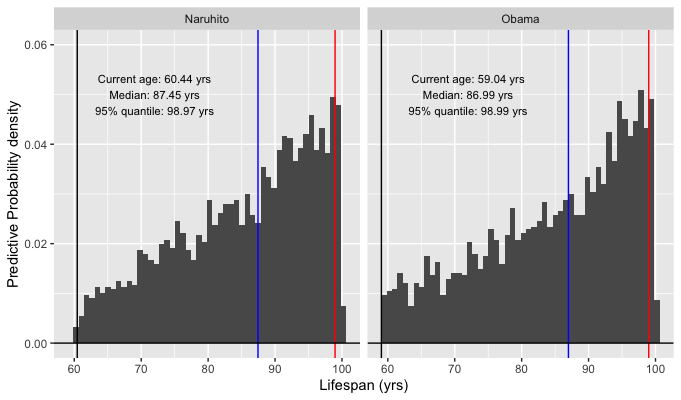
\includegraphics{/Users/cathylee/Documents/Course Folders/Fall 2020/STA 440/Case 1/case_study_one/naru_obama_pp.png}
=======
>>>>>>> ff2267c030cf7f5179303b8ed9d679345292487f

The posterior predictive distribution of the lifespan of the 14th Dalai
Lama is more uniform, with mode in the 90s. The posterior predictive
distribution of the lifespan of Pope Francis is somewhat left skewed,
with the mode in the early 90s. The posterior predictive distributions
of the lifespans of President Obama and Emperor Naruhito are both left
skewed, with the modes in the late 90s.

The probability that the 14th Dalai Lama will have a longer lifespan
than Pope Francis is 0.495. The probability that President Obama will
have a longer lifespan than Emperor Naruhito is 0.483.

\hypertarget{vi.-conclusion-and-further-discussion}{%
\section{VI. Conclusion and Further
Discussion}\label{vi.-conclusion-and-further-discussion}}

\hypertarget{vii.-appendix}{%
\section{VII. Appendix}\label{vii.-appendix}}

<<<<<<< HEAD
=======
<<<<<<< HEAD

=======
>>>>>>> f3f68c29bd121ea31a42eb9f939b261bd39569de
>>>>>>> ff2267c030cf7f5179303b8ed9d679345292487f
\end{document}
